\chapter{Linear Systems}
\section{Intersections as a Concept}

An important idea in math is the idea of a set.  Sets are collections of objects.  We can talk about the set of flowers, the set of things that are red, or whatever other category of thing we can think of.  If something belongs to both sets, we say that it is in the intersection of those sets.


\begin{prblm}
What's something that's in the intersection of the set of flowers and the set of things that are red?
What would the intersection of the solution sets of two linear equations be like?
\vspace{5cm}
\end{prblm}


We've briefly mentioned sets before.

Recall: What is the solution set for the line $y=-x$? What about the line $y=2x+1$?


\begin{defn}[Linear System]
A linear system is made up of multiple linear equations. The solution set for a linear system is the intersection of the solution sets of the linear functions. 
\end{defn}

Over the course of the past few sections, we've been reinforcing this idea that plotting a linear equation as a line makes some features easier to see, such as other solutions, and overall trends of those solutions.  Furthermore, finding the equation that goes with a line that has been plotted gives us some extra power, such as the ability to find solutions that are outside of the plot, or express the facts of the situation in words so that we can communicate these ideas more easily.

\begin{defn}[Consistent System]
We call a linear system consistent if and only if there exists a solution.	
\end{defn}

\begin{prblm}
Find some solutions to the equation $y = 3 - x$.
Find some solutions to the equation $y = 2x$.

How would you find the intersection of their solution sets?

\vspace{5.5cm}
\end{prblm}

However, there are some lines that do not intersect.

\begin{defn}[Parallel Lines]
We call two lines with the same slope parallel lines. If two lines are parallel, they will never intersect. Likewise, if two lines intersect, then they are not parallel. 	
\end{defn}
This is an important definition to remember, especially when we are dealing with graphing two separate lines on the same graph.

\begin{defn}[Inconsistent System]
We call a linear system inconsistent when there is no point of intersection (no solution).	
\end{defn}

\begin{theorem}[Solutions of a Linear System]
There is either a single solution, no solution, or infinite solutions to a linear system with two equations. 	
\end{theorem}

\noindent
\textbf{\underline{Evidence}:} Consider the possibilities for two lines in a linear system. The first case is they intersect. To see an example, flip back to Example 1.4. Since lines remain straight, they will never intersect again. There is our first case (a single solution). If they don't intersect, then Definition 1.6 tells us that they must be parallel. In most cases, if two lines are parallel, then the system will have no solution, since there is no point in which they will intersect, confirming our second case (no solution). Finally, there is one particular case that we have not mentioned yet. If two lines are equivalent, then the solution set will be infinitely large, since every point will intersect, which gives us our last result (infinite solutions). Thus, the theorem is true. 
\pagebreak

\section{Graphing Linear Systems}

We've mentioned before that a coordinate system can be created with any scale we want.  The $x$ and $y$ axes don't even need to have the same scale.  That idea requires some refinement now: if we put two lines on the same coordinate system, we have to use them same scale for each line.  When we do this, if we're plotting the line from a set of points, we need to make sure we finish plotting the first line before moving on to the second.

%Insert Illustration

\begin{figure}[ht] 
  \label{ fig7} 
  \begin{minipage}[b]{0.5\linewidth}
    \centering
    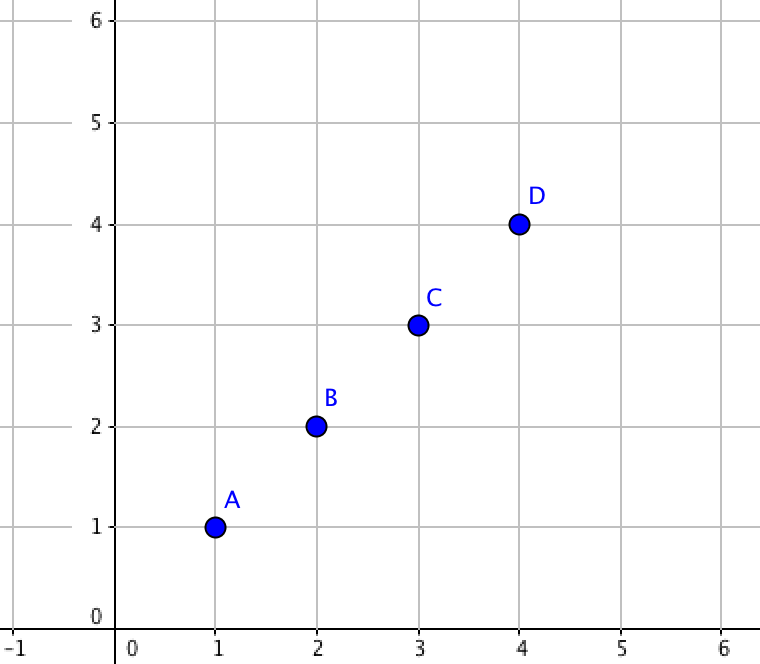
\includegraphics[width=.5\linewidth]{points.png} 
    \caption{Plotting points for the line $y=x$.} 
    \vspace{4ex}
  \end{minipage}%%
  \begin{minipage}[b]{0.5\linewidth}
    \centering
    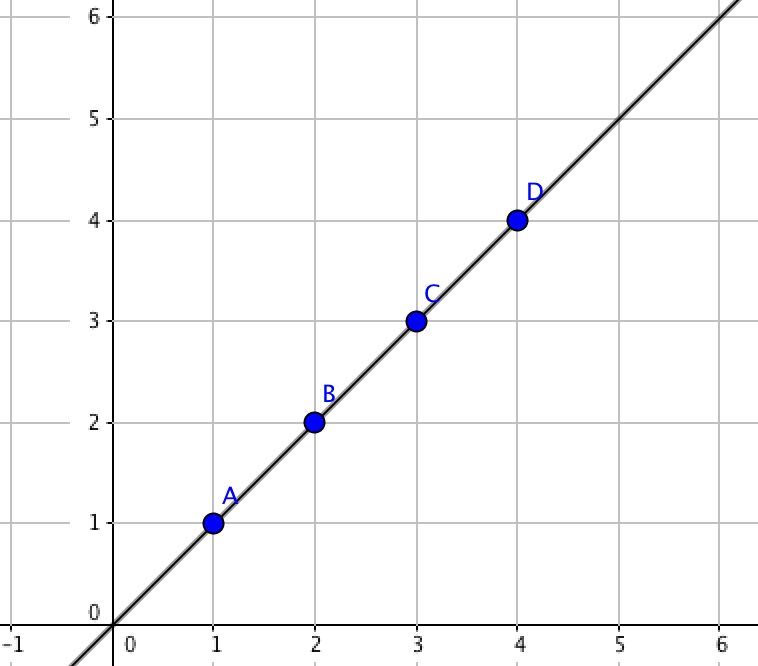
\includegraphics[width=.5\linewidth]{pointsline.png} 
    \caption{The line $y=x$.} 
    \vspace{4ex}
  \end{minipage} 
  \begin{minipage}[b]{0.5\linewidth}
    \centering
    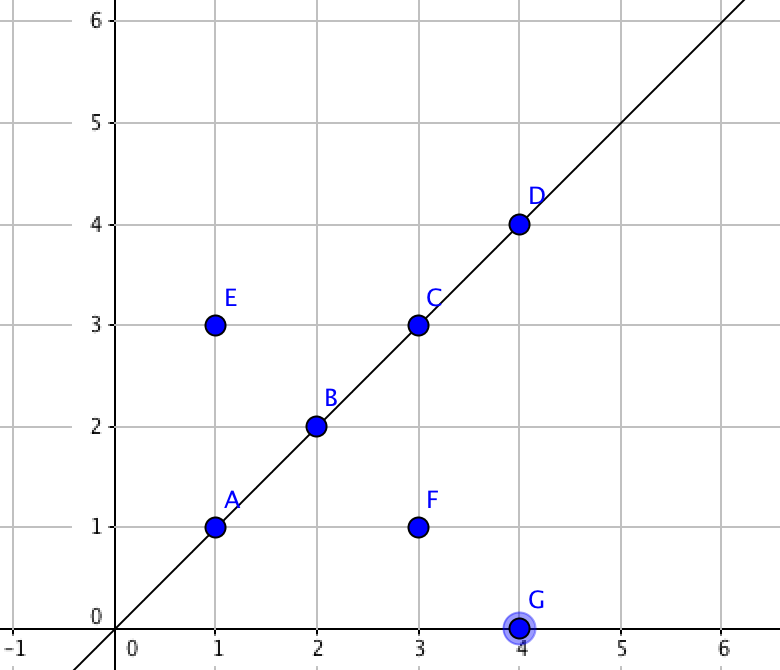
\includegraphics[width=.5\linewidth]{points2.png} 
    \caption{Plotting points for a new line.} 
    \vspace{4ex}
  \end{minipage}%% 
  \begin{minipage}[b]{0.5\linewidth}
    \centering
    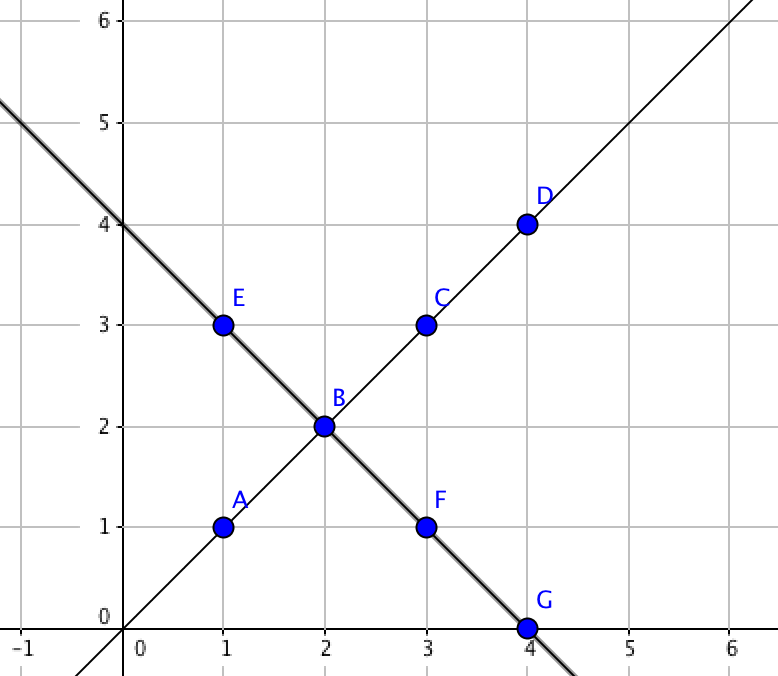
\includegraphics[width=.5\linewidth]{line2.png} 
    \caption{The lines $y=x$ and $y=-x+4$.} 
    \vspace{4ex}
  \end{minipage} 
\end{figure}


It's no coincidence that we call the objects in two sets the ``intersection''.  A single solution in the solution set of an equation is a point on the line that corresponds to that equation.  If we have two lines on a graph, the point where they intersect is a point that's on both of the lines at the same time.  That means that the point is going to be in the solution set of both equations.

\begin{example}
Find the intersection for the following system of linear equations.
$$y - 4x = -4$$
$$2y + x = 10$$

Using this strategy, we want to plot both equations.  To do this, we want them in a form that we can use to plot them, so we'll put them in slope-intercept form.
For the first line:
$$
\begin{array}{rcl}
y - 4x & = & -4 \\
y & = & 4x - 4 \end{array}$$

And for the second line:
$$\begin{array}{rcl}
2y + x & = & 10 \\
2y & = & 10 - x \\ 
y & = & 5 - \frac{x}{2} \\
y & = & - \frac{1}{2} x + 5 \end{array}$$

Plotting both lines then shows that they have an intersection.
%Insert graph
\begin{center}
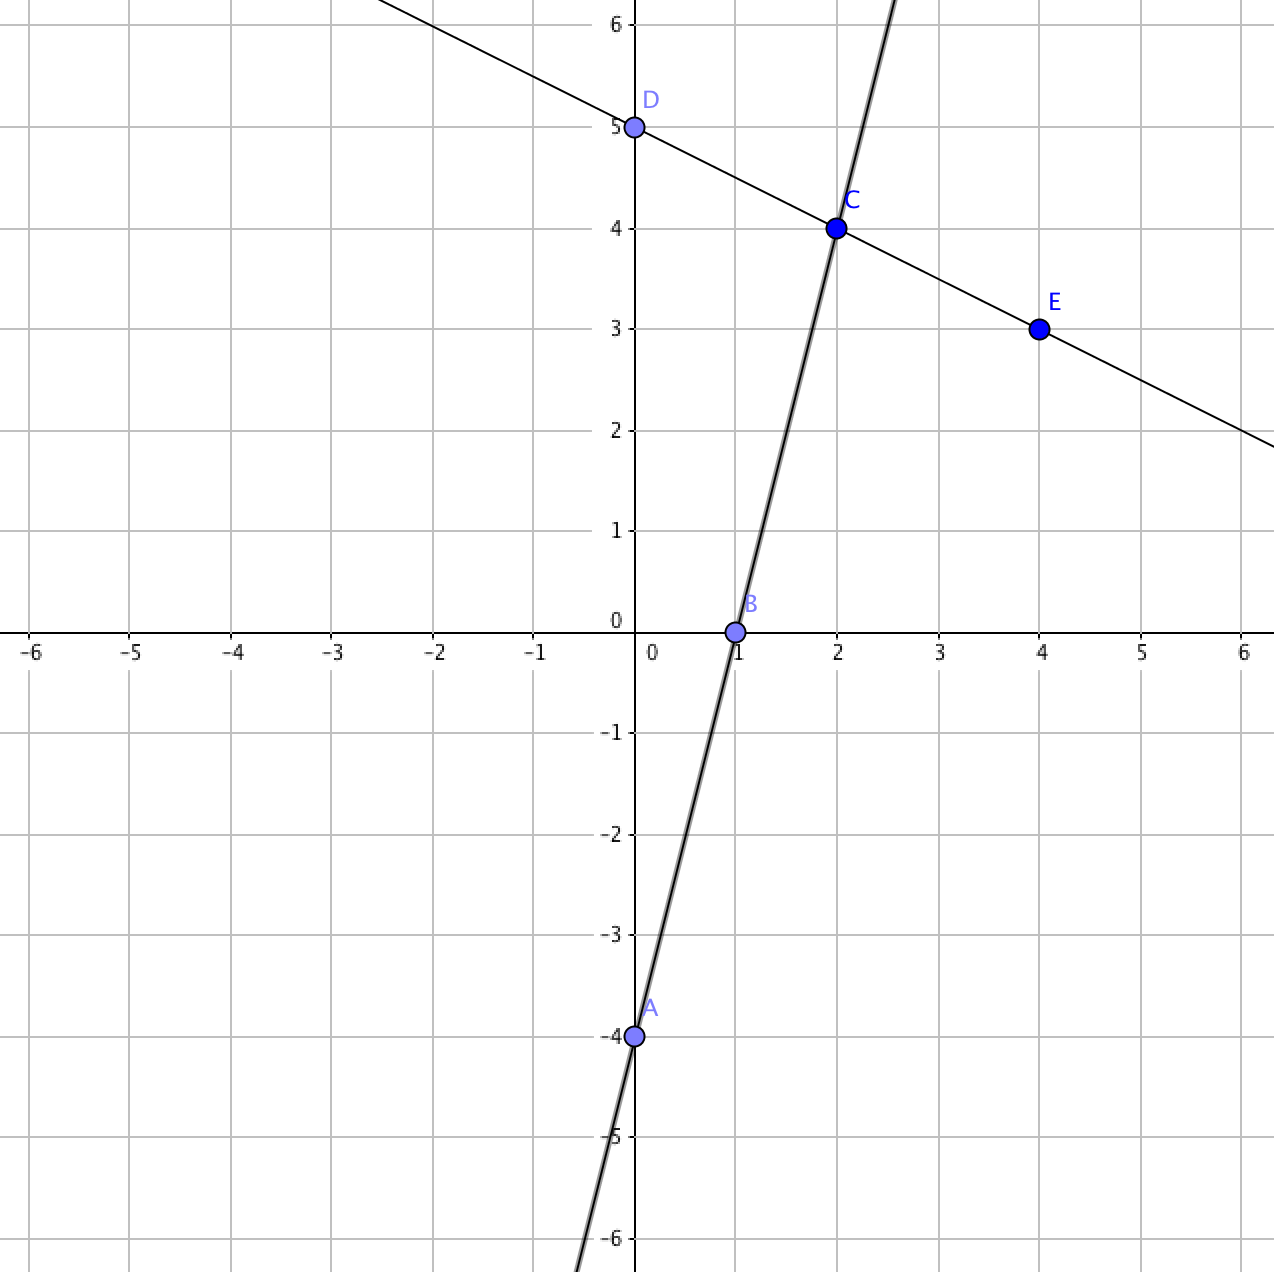
\includegraphics[scale=.35]{intersection.png}	
\end{center}

We can then see that the lines intersect at the point $(2,4)$.  This means that $(2,4)$ is in the solution set to both equations, and is thereby the solution to this system of equations.
\end{example}

This is a useful tool for finding solutions to systems of linear equations as long as being close is good enough.  Unfortunately, some systems of linear equations have solutions that aren't on the grid-lines for a particular scale.

\begin{prblm}
Consider the following system of linear equations.
$$y = -\frac{1}{2}x + 3$$
$$y = 2x$$

What do you think the intersection is?  What could you do to convince someone who didn't agree?

\vspace{4cm}
\end{prblm}


\section{Substitution}

Although most people aren't accustomed to the idea, there is more than one way to do most things in math.  This is a good thing!  If the only way to find the solution to a system of equations was to graph them and point at it, it would be pretty difficult to solve a lot of these systems.  This is where substitution comes in.  Consider two equations in slope-intercept form.

$$y = 2x + 4$$
$$y = 3x + 2$$

If we were to find a solution to this system of equations, there would only be one $y$-value, and it would apply for both of the equations.  In other words, we know that $y$ will have the same value for each equation.  Let's say we know that the solution has a $y$-value of $8$.  We would then have, 

$$8 = 2x + 4$$
$$8 = 3x + 2$$

Well, if the right side of the first equation is equal to $8$, and the right side of the second equation is equal to $8$, they must be equal to each other!  This is the driving force of substitution.  If two things have the same value, they're equal to each other.

$$2x + 4 = 3x + 2$$

And this is single linear equation like we had in the second unit!  We can solve this.

$$\begin{array}{rcl}
2x + 4 & = & 3x + 2\\
4 & = & x + 2 \\
2 $ = $ x \end{array}$$

So now we know the solution has an $x$-value of $2$.  Nice.  So what about that $y$-value?  Is it really $8$?  We can plug the $x$-value we just found into one of those equations and find out.  We'll choose the first equation.

$$\begin{array}{rcl}
y & = & 2\times2 + 4\\
y & = & 4 + 4\\
y & = & 8 \end{array}$$

Awesome.  Now we think the solution has an $x$-value of $2$, and a $y$-value of $8$.  If this is true, then $(2,8)$ must be a solution to the second equation as well.  We can check that.

$$\begin{array}{rcl}
y & = & 3x + 2 \\
8 & = & 3\times 2 + 2\\
8 & = & 6 + 2 \end{array}$$

Everything checks out.  We've found a solution to this linear system.

\pagebreak
\begin{prblm}
Try using the graphing strategy on this linear system.  Compare the results.

\begin{center}
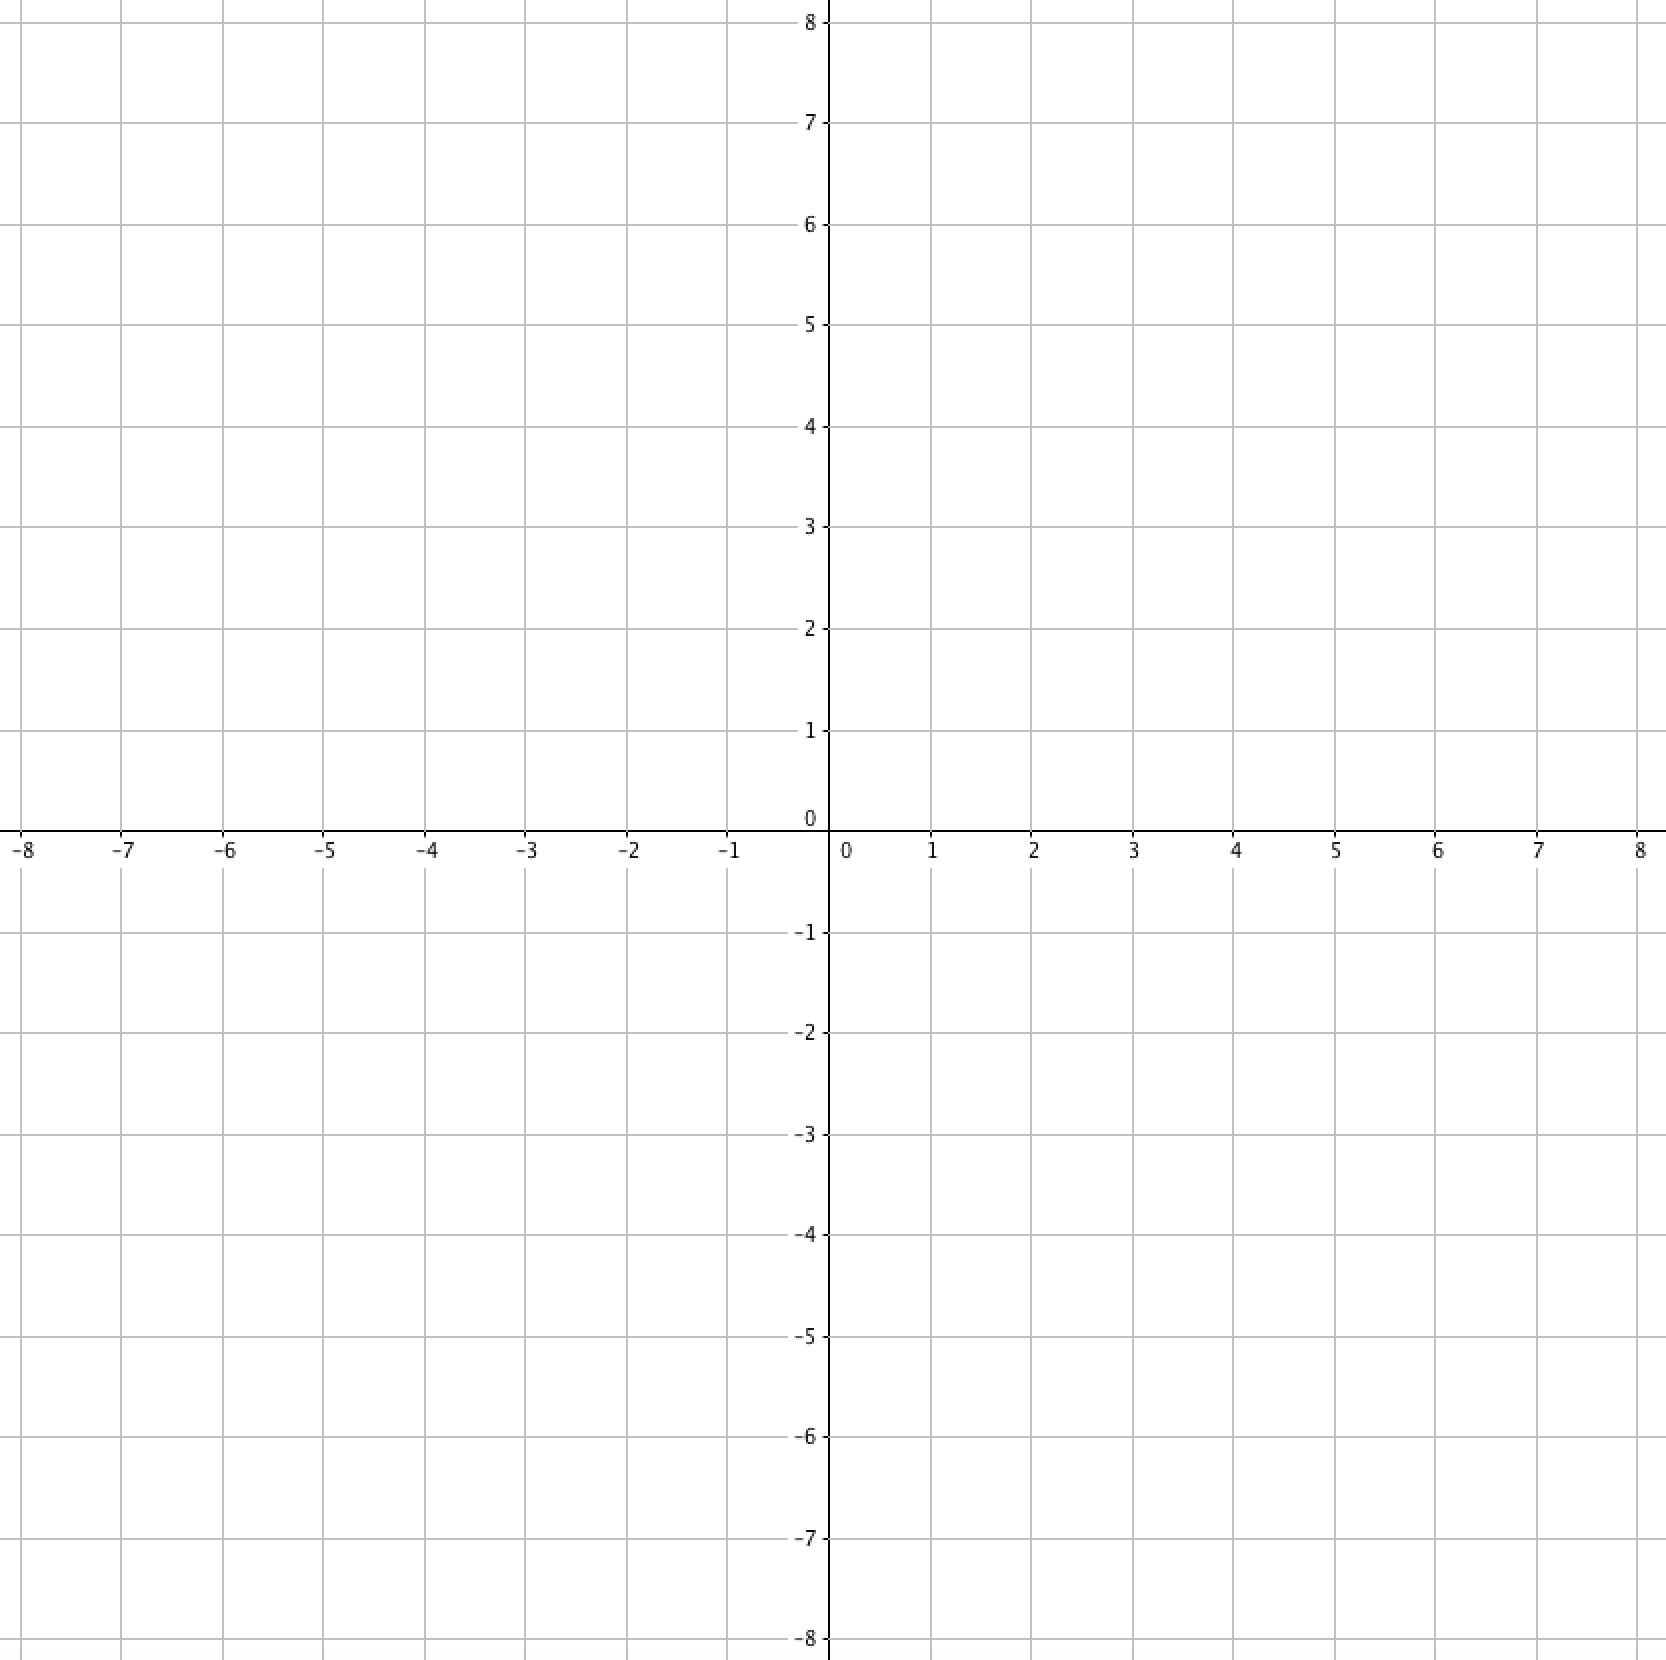
\includegraphics[scale=.4]{blank.png}	
\end{center}

\end{prblm}

For this last problem, the solution had nice, clean integer values for the solution.  The equations were also given in slope-intercept form.  This won't always be the case.

\begin{example}
Solve the system of linear equations.

$$\begin{array}{rcl}
4y - 16x & = & 25 \\
2y + x & = & -1 \end{array}$$

To use the substitution strategy the way we did last time, we want to solve each equation for either $y$ or $x$.  We had the equations solved for $y$ last time, and solving for $y$ should be natural to us by now, so we'll do that for now.

For the first equation:

$$\begin{array}{rcl}
4y - 16x & = & 25 \\
4y & = & 16x + 25 \\
y & = & 4x + \frac{25}{4} \end{array}$$

And for the second equation:

$$\begin{array}{rcl}
2y + x & = & -1 \\
2y & = & -x -1 \\
y & = & -\frac{1}{2}x - \frac{1}{2} \end{array}$$

Now we're in a similar position as we were at the beginning of the last problem.  We realize that both $-\frac{1}{2}x - \frac{1}{2}$ and $4x + \frac{25}{4}$ are equal to $y$, and so we set them equal to each other.

$$\begin{array}{rcl}
-\frac{1}{2}x - \frac{1}{2} & = & 4x + \frac{25}{4}\\ \\
-\frac{1}{2} & = & 4\frac{1}{2}x + \frac{25}{4}\\ \\
-\frac{1}{2} - \frac{25}{4} & = & 4\frac{1}{2}x\\ \\
-\frac{2}{4} - \frac{25}{4} & = & \frac{9}{2}x\\ \\
-\frac{27}{4} & = & \frac{9}{2}x\\ \\
-\frac{27}{4} \div \frac{9}{2}& = & x \\ \\
-\frac{3}{2} & = & x\\
\end{array}$$

So we've figured out that the solution has an $x$-value of $-\frac{3}{2}$.  Now we need to figure out the $y$-value.  Again, we plug our $x$-value into one of the equations, and the $y$-value should come out.  The great part is that, for the whole sequence where we solved for $y$ in the first equation, each of those equations is equivalent.  We can choose the new version of the first equation to find our $y$-value.

$$\begin{array}{rcl}
y & = & 4\times \left(-\frac{3}{2}\right) + \frac{25}{4}\\
y & = & -\frac{12}{2} + \frac{25}{4}\\
y & = & -\frac{24}{4} + \frac{25}{4}\\
y & = & \frac{1}{4}\\
\end{array}$$

This tells us that the point in the first equation where the $x$-value is $-\frac{3}{2}$ has a $y$-value of $\frac{1}{4}$.  Then, the solution is the point, $\left(-\frac{3}{2}, \frac{1}{4}\right)$.
\end{example}

Let's try a tougher one.

\begin{example}
Solve the system of linear equations.
$$2y - 3x = 9$$
$$5y + 2x = -10$$

For the first equation:

$$\begin{array}{rcl}
2y - 3x & = & 9\\
2y & = & 3x + 9\\
y & = & \frac{3}{2}x + \frac{9}{2} \end{array}$$

And for the second equation:

$$\begin{array}{rcl}
5y + 2x & = & -10\\
5y & = & -10 - 2x\\
y & = & -\frac{2}{5}x - 2 \end{array}$$

Now, setting the right side of each equation equal, 

$$\begin{array}{rcl}
\frac{3}{2}x + \frac{9}{2} & = & -\frac{2}{5}x - 2\\ \\
\frac{3}{2}x + \frac{2}{5}x + \frac{9}{2} & = & - 2\\ \\
\frac{3}{2}x + \frac{2}{5}x & = & -\frac{9}{2} - 2\\ \\
\frac{15}{10}x + \frac{4}{10}x & = & -\frac{9}{2} - \frac{4}{2}\\ \\
\frac{19}{10}x & = & -\frac{13}{2}\\ \\
x & = & -\frac{13}{2} \div \frac{19}{10}\\ \\
x & = & -\frac{65}{19} \\
\end{array}$$
\end{example}


\section{Elimination}

There's yet another strategy for solving systems of linear equations.  This strategy is based on a similar idea as the one the substitution strategy is based on.  Both sides of an equation are equal, and can be replaced with the other.  Consider the following linear system.

$$\begin{array}{rcl}
y - x & = & 4 \\
y + x & = & 2\end{array}$$

From the second unit, we learned that, as long as we add the same thing to both sides, the equation will still be equivalent.  For this strategy, we want to take advantage of the fact that each side of the first equation has the same value.  If we think of the equations as balanced scales, we can think of our next step as taking everything off of the second scale and putting it on the appropriate sides of the first scale.

$$\begin{array}{rcl}
y - x & = & 4 \\
y - x + (y + x) & = & 4 + (2)
\end{array}$$

The stuff in parentheses comes from the second equation.  At this point, we just want to simplify and see what happens.

$$\begin{array}{rcl}
y - x + (y + x) & = & 4 + (2)\\
y - x + y + x & = & 6\\
2y + 0x & = & 6\\
2y = 6
y = 3 \end{array}$$

What happened?

When we took everything from the second equation and put it on the first, we ended up with an equation that has a solution where both of our previous equations had solutions.  Since this value only has a $y$-value and no $x$-value, we have the beginning of a solution!  Let's put that $y$-value in and see what $x$ is.

$$
\begin{array}{rcl}
y - x & = & 4 \\
3 - x & = & 4 \\
3 & = & 4 + x \\
-1 & = & x \end{array}$$

With a value $y$ and $x$, we have a complete solution.  We call this the Elimination Method because the hope is that, when we add the equations together, one of the variables will cancel or be eliminated, leaving us with a linear equation with only one variable.  This worked out for us this time because one equation had a positive $x$, and the other equation had a negative $x$.  If we have more $x$'s in one equation than the other, we'll have some positive or negative $x$'s left over.  In order to make them cancel, we sometimes have to find an equivalent equation.

\begin{example}
Solve the following linear system using the elimination method.

$$\begin{array}{rcl}
y + 2x & = & -2\\
-2y - x & = & 3 \end{array}$$

If we take the second equation and add it to the first equation now, we'll still have an equation with two variables.

$$\begin{array}{rcl}
y + 2x + (-2y - x) & = & -2 + (3)\\
y + 2x - 2y - x & = & 1\\
-y + x & = & 1 \end{array}$$

Like before, we ended up with an equation that has a solution where both of our previous equations had solutions. Unfortunately, it still has two variables, so we can't make any conclusions about it yet.  Let's take a look at the first two equations again.  Notice that the second equation has only one negative $x$, while the first equation has two.  We want to take advantage of equivalent equations.  If we want an equation equivalent to the second equation, but which has two negative $x$'s, we can multiply both sides by 2. Then, the system

$$\begin{array}{rcl}
y + 2x & = & -2\\
-2y - x & = & 3 \end{array}$$

becomes

$$\begin{array}{rcl}
y + 2x & = & -2\\
-4y - 2x & = & 6 \end{array}$$

Because the equations we have are equivalent to the previous equations, the linear system is also equivalent; it will have all of the same solutions.  Let's try adding the equations again.

$$\begin{array}{rcl}
y + 2x + (-4y - 2x) & = & -2 + (6) \\
y + 2x -4y -2x & = & 4 \\
-3y & = & 4 \\
y & = & -\frac{4}{3}
\end{array}$$

Perfect.  We eliminated one of the variables according to plan.  We know that our solution has a $y$-value of $-\frac{4}{3}$.  We can work on finding $x$ now.  This will be easier if we start with the second equation, so we don't have to divide at the end.

$$\begin{array}{rcl}
-2y - x & = & 3 \\
-2\times \left(-\frac{4}{3}\right) - x & = & 3 \\
\frac{8}{3} - x & = & 3 \\
\frac{8}{3} & = & 3 + x \\
\frac{8}{3} - 3 & = & x \\
\frac{8}{3} - \frac{9}{3} & = & x \\
-\frac{1}{3} & = & x \end{array}$$

With values for $x$ and $y$, we can now say that we have a solution.
\end{example}

We're going to do one more example, but there's going to be a twist to it.

\begin{example}
Solve the system of linear equations.

$$\begin{array}{c}
y = \frac{3}{5}x - 6\\
3y + 2x = 1 \end{array}$$

The first thin we have to watch out for is the equals sign.  Remember that the strategy only works because we're taking everything off of one scale and putting it on the appropriate sides of the other scale.  We can't add straight down because the equals signs don't line up.  We have to make sure they do.

$$\begin{array}{rcl}
y & = & \frac{3}{5}x - 6\\
3y + 2x & = & 1 \end{array}$$

That's better.  Now we can clearly see that we need to move the $\frac{3}{5}x$ term to the other side of the first equation.

$$\begin{array}{rcl}
y - \frac{3}{5}x & = & -6\\
3y + 2x & = & 1 \end{array}$$

Now we're in a weird spot.  It looks like we would have to multiply one of the equations by a fraction in order to get the $x$'s to cancel.  Finding that fraction can sometimes take valuable time.  What we're going to do is take advantage of equivalent equations again, and we're going to fix both of the equations.  We'll look at the coefficient of the $x$ in the first equation, and multiply the second equation by it.  Then we'll look at the coefficient of $x$ in the second equation and multiple by first equation by it.  This way, the $x$'s in both equations will be multiplied by both coefficients, and this should make them cancel.


$$\begin{array}{rcl}
y - \frac{3}{5}x & = & -6\\
3y + 2x & = & 1\\ \\
y - \frac{3}{5}x & = & -6\\
\frac{3}{5}\times 3y + \frac{3}{5}\times 2x & = & \frac{3}{5}\times 1\\ \\
y - \frac{3}{5}x & = & -6\\
\frac{9}{5}y + \frac{6}{5}x & = & \frac{3}{5}\\ \\
2y - 2\times \frac{3}{5}x & = & 2\times (-6)\\
\frac{9}{5}y + \frac{6}{5}x & = & \frac{3}{5}\\ \\
2y - \frac{6}{5}x & = & -12 \\
\frac{9}{5}y + \frac{6}{5}x & = & \frac{3}{5} \end{array}$$

And now, when we add the equations together, the $x$'s will cancel.

$$\begin{array}{rcl}
2y - \frac{6}{5}x + (\frac{9}{5}y + \frac{6}{5}x) & = & -12 + (\frac{3}{5}) \\
2y - \frac{6}{5}x + \frac{9}{5}y + \frac{6}{5}x & = & -\frac{60}{5} + \frac{3}{5} \\
2y + \frac{9}{5}y & = & -\frac{57}{5} \\
\frac{10}{5}y + \frac{9}{5}y & = & -\frac{57}{5} \\
\frac{19}{5}y & = & -\frac{57}{5} \\
y & = & -\frac{57}{5} \div \frac{19}{5}\\
y & = & -3
\end{array}$$

We have a $y$-value.  What's missing?

$$\begin{array}{rcl}
3y + 2x & = & 1\\
3 \times -3 + 2x & = & 1 \\
2x & = & 10 \\
x & = & 5 \end{array}$$

This tells us that our solution is $(5,-3)$.
\end{example}

As we can see, some problems are more well-suited for elimination than others.

\begin{prblm}
Would it be easier to solve this problem with the graphing, substitution, or elimination strategies?
How would you be able to tell before trying any of them?
\end{prblm}


